\documentclass{ximera}
%\usepackage{todonotes}

\usepackage{tkz-euclide}
\usetikzlibrary{backgrounds} %% for boxes around graphs
\usetikzlibrary{shapes,positioning}  %% Clouds and stars
\usetkzobj{all}
\usepackage[makeroom]{cancel} %% for strike outs
%\usepackage{mathtools} %% for pretty underbrace % Breaks Ximera
\usepackage{multicol}


\newcommand{\RR}{\mathbb R}
\renewcommand{\d}{\,d}
\newcommand{\dd}[2][]{\frac{d #1}{d #2}}
\renewcommand{\l}{\ell}
\newcommand{\ddx}{\frac{d}{dx}}
\newcommand{\zeroOverZero}{$\boldsymbol{\tfrac{0}{0}}$}
\newcommand{\numOverZero}{$\boldsymbol{\tfrac{\#}{0}}$}
\newcommand{\dfn}{\textbf}
\newcommand{\eval}[1]{\bigg[ #1 \bigg]}
\renewcommand{\epsilon}{\varepsilon}
\renewcommand{\iff}{\Leftrightarrow}

\DeclareMathOperator{\arccot}{arccot}
\DeclareMathOperator{\arcsec}{arcsec}
\DeclareMathOperator{\arccsc}{arccsc}


\colorlet{textColor}{black} 
\colorlet{background}{white}
\colorlet{penColor}{blue!50!black} % Color of a curve in a plot
\colorlet{penColor2}{red!50!black}% Color of a curve in a plot
\colorlet{penColor3}{red!50!blue} % Color of a curve in a plot
\colorlet{penColor4}{green!50!black} % Color of a curve in a plot
\colorlet{penColor5}{orange!80!black} % Color of a curve in a plot
                                      \colorlet{fill1}{blue!50!black!20} % Color of fill in a plot
\colorlet{fill2}{blue!10} % Color of fill in a plot
\colorlet{fillp}{fill1} % Color of positive area
\colorlet{filln}{red!50!black!20} % Color of negative area
\colorlet{gridColor}{gray!50} % Color of grid in a plot

\pgfmathdeclarefunction{gauss}{2}{% gives gaussian
  \pgfmathparse{1/(#2*sqrt(2*pi))*exp(-((x-#1)^2)/(2*#2^2))}%
}



\newcommand{\fullwidth}{}
\newcommand{\normalwidth}{}



%% makes a snazzy t-chart for evaluating functions
\newenvironment{tchart}{\rowcolors{2}{}{background!90!textColor}\array}{\endarray}

%%This is to help with formatting on future title pages.
\newenvironment{sectionOutcomes}{}{} 

\author{Emma Smith Zbarsky}
\license{Creative Commons Attribution 3.0 Unported}
\acknowledgement{https://quadbase.org/questions/q14361v1}
\begin{document}

\begin{exercise}

Consider the equation \[\sqrt{x^2+y^2} = 3\sin(3x+y).\] A graph of the
solutions to this implicitly defined function is shown here:


\begin{image}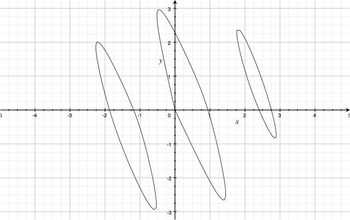
\includegraphics[width=.5\textwidth]{implicitcurve.jpg}\end{image}



Calculate $\frac{dy}{dx}$ using implicit differentiation for this curve,
and determine what the domain of the function $y(x)$ is.


\begin{multipleChoice}
\choice{$\frac{dy}{dx} = \frac{9\cos(3x+y)\sqrt{x^2+y^2}-x}{y}$ Domain is
$[-\sqrt{3},\sqrt{3}]$.}
\choice[correct]{$\frac{dy}{dx} =  \frac{9\cos(3x+y)\sqrt{x^2+y^2}-x}{y-3\cos(3x+y)\sqrt{x^2+y^2}}$
Domain is $[-\sqrt{3},\sqrt{3}]$.}
\choice{$\frac{dy}{dx} = -\frac{x+9\cos(3x+y)\sqrt{x^2+y^2}}{3\cos(3x+y)\sqrt{x^2+y^2}+y}$
Domain is $[-\sqrt{3},\sqrt{3}]$.}
\choice{$\frac{dy}{dx} =  \frac{3\cos(3x+y)\sqrt{x^2+y^2}-x}{y-3\cos(3x+y)\sqrt{x^2+y^2}}$
Domain is $[-3,3]$.}
\choice{$\frac{dy}{dx} = \frac{9\cos(3x+y)\sqrt{x^2+y^2}-2x}{2y-3\cos(3x+y)\sqrt{x^2+y^2}}$
Domain is $[-3,3]$.}
\end{multipleChoice}

\end{exercise}
\end{document}
